\documentclass[12pt, letterpaper]{article}
\usepackage[utf8]{inputenc}
\usepackage{mathptmx}
\usepackage{geometry}
\usepackage{siunitx}
\usepackage{appendix}
\usepackage{pdfpages}
\usepackage{amsmath, amsthm, amssymb}
\usepackage{minted}
\usepackage{booktabs}
\geometry{a4paper, margin=1in}

\usepackage{graphicx}
\usepackage{setspace}
\doublespacing

\usepackage[style=numeric, backend=biber, sortcites=true, sorting=nyt]{biblatex}
\addbibresource{references.bib}
\usepackage{titlesec}
\usepackage{fancyhdr}
\pagestyle{fancy}
\fancyhead[L]{Fancy Head} 
\fancyhead[R]{\thepage} 
\fancyfoot{} % Clear all footer settings
\renewcommand{\headrulewidth}{0pt}

\begin{document}

\begin{titlepage}
    \centering
    \Large\textbf{IE University}\\[0.5cm]
    \large\textit{School of Science \& Technology}\\[1.5cm] 
    
\includegraphics[width=0.4\textwidth]{graphics/SST.png}\\ 
    \Huge\textbf{Hybrid Quantum-Classical Software Stack for HPC Algorithm Acceleration}\\[0.5cm] 
    % \LARGE\textit{Subtitle of the project}\\[1cm] 
    \Large\textbf{Anna Payne}\\ 
    \large\textit{Bachelor of Computer Science \& Artificial Intelligence}\\[0.5cm] 
    \Large\textit{Supervised by:}\\
    \Large\textbf{Prof. Oscar Diez}\\ 
    \large\textit{Robotics \& AI Lab, School of Science \& Technology, IE University, Spain}\\[1cm] 
\end{titlepage}




\begin{abstract} 
With the evolution of quantum processing units (QPUs) as specialized accelerators, integrating quantum kernels into High Performance 
Computing (HPC) systems has been increasing explored within the field of computational science. Hybrid quantum-classical systems have 
gained researchers attention by their combination of the strength of both computational paradigms in a method to overcome current 
quantum hardware limitations, specifically regarding qubit coherence and error rates. An example is the Variational Quantum Eigensolver 
(VQE), an algorithm which offloads the computationally intensive optimization loop to its classical computing resources, 
while allowing the QPUs to exclusively handle the execution of quantum circuits and the measurement of resulting expectation values. 
In present day, there is a lack of existing unified middleware that is constructed to bridge the low latency QPU control with 
HPC infrastructures, so for that reason the development of this middleware will focus on three objectives: designing an 
accesible API to abstract the cloud based QPU backend's complexity, the development of HPC connectors using MPI/CUDA in order to 
parallelize the classical subroutines, and a performance analysis of the software framework using VQE workflows. The stack's 
evaluation will occur on a single Docker host and laptop GPU with the primary objective of a 1.5x speedup in end-to-end wall-clock time 
as when compared to nonoptimized implementations, with the architecture supporting future gains on HPC hardware. In this work, we aim at the development of a accesible, 
open-source framework that will provide a measureable speedup in hybrid quantum-classical simulations for future usage in fields 
such as materials science or complex optimization, specificallymul in a user-friendly manner to ensure accesibility for non-programming or 
non-quantum experts. 


\noindent\textbf{Keywords:} Quantum Systems, Hybrid Systems, Variational Quantum Eigen-solver, High-Performance Computing, 
Algorithm Acceleration, MPI, CUDA, Software Middleware.
\end{abstract}




\section{Introduction}
    The field of High Performance Computing (HPC) has been undergoing a transformation towards heterogeneous architectures 
    that are not defined by the sole usage of CPUs. In past decades, the integration of General Purpose Graphic 
    Processing Units (GPGPUs) alongside Central Computing Units (CPUs) have defined the limits of this field's 
    computational power. However in recent years, there has been a rising demand for more advanced systems that have the ability to stimulate
    complex molecular dynamics and combinatorial optimization, shining a light on our current classical computational limitations. 
    Issues such as the curse of dimensionality and the exponential scaling of Hilbert space have redirected this field's focus 
    towards the potential advantages of Quantum Processing Units (QPUs).  QPUs have emerged, not to be the replacement for classical computation, but 
    instead as specialized accelerators that will be integrated into our existing classical systems, as these processing units are capable of handing 
    specific computational tasks that are intractable for classical bits ~\cite{rallis2025interfacingquantumcomputingsystems}. However, quantum technology 
    is a new advancement, one that still needs significant refinement and testing due to their current limitations. 
    This means hybrid frameworks are the current industry goal to work towards in the hopes of achieving new ground within the fields of material science, 
    drug discovery, complex optimization, cryptographic analysis, and many others.  

    Currently, we are in the era of Noisy Intermediate-Scale Quantum (NISQ), where quantum hardware is limited and noisy, 
    unable to harness the true potential of a "quantum advantage" \cite{harrow2017quantumsupremacy}. The most promising path of achieving this 
    is hybrid quantum-classical algorithms ~\cite{rallis2025interfacingquantumcomputingsystems} that combine the computational benefits of each system. 
    Specifically algorithms such as Variational Quantum Eigensolver (VQE), containg a feedback loop that 
    a classical optimizer uses to iteratively refine parameters to be entered into the connected quantum circuit. By offloading a computationally heavy optimization loop to (heterogeneous) classical 
    resources, QPUs prioritze executing circuits and measuring the resulting expectation values, allowing developers  
    to bypass current QPU coherency limitations which leave us with incorrect and decolorant results. However, if long term coherency is achieved, various quantum algorithms could 
    provide us with an exponential speedup over classical methods when determining eigenvalues in large and complex problems ~\cite{peruzzo2014variational}. 
    Classical HPC structures that use MPI, CUDA and GPUs all in dense, parallelized numerical workloads and larger 
    scale simulations, however struggle when the problem dimension grows exponentially alongside 
    the size of the physical system being observed. This issue is present when calculating the arrangement and behavior of electrons in a molecule, but can be addressed 
    by hybrid systems, leaving quantum components to map the wavefunction directly onto qubits while the classical 
    components refine the variational parameters for circuits \cite{rallis2025interfacingquantumcomputingsystems}.
    
    Despite the theoretical potential of hybrid collaboration, this field currently has a significant architectural gap, as  
    there is a lack of specialized middleware that bridges quantum and classical components. Classical HPC frameworks (ones that are optimized 
    for MPI and CUDA) are not designed to communicate directly with quantum control stacks or hardware. This requires quantum researchers and developers to manually handle the complex 
    data serialization and the frequent network latencies that occur in this communication. Existing quantum programming frameworks, such as Qiskit and Cirq, 
    excel with circuit-level QPU control but lack features to effectively integrate with distributed HPC environments, lacking the ability to seamlessly  
    communicate between the two systems. Without the existence of a standardized hybrid middleware, quantum researchers are facing issues such as high tail latencies that are observed when synchronizing
    both HPC nodes and cloud-based QPUs, leading to performances bottlenecks that ruins the possibility of a speedup offered by a
    hybrid system. This issue, combined with the complex task of data serialization for quantum hardware and the potential lack of understanding of the intricate communication  
    between quantum and classical systems, leaves a difficult barrier for researchers to overcome. 

    The proposed project that this paper will undertake is the development of a hybrid quantum-classical software stack that builds the middleware layer needed
    to abstract hardwares and automate the dispatching of tasks. This software stack will design a clear, intuitive API that will abstract the 
    backend of the cloud-based QPU, removing the need for quantum researchers or developers to manually handle the communication complexities in a hybrid system. This hybrid stack 
    will include automated dispatching logic, HPC connectors to the Qiskit framework, and classical kernels 
    that use MPI and CUDA to parallelize the classical optimization subroutines for an added speedup. The stack is benchmarked against VQE workflows 
    on a single host Docker environment alongside MPI/GPU acceleration, aiming to demonstrate measurable progress towards the "quantum advantage," with a 1.5x 
    speedup in the end-to-end wall-clock time when being compared to the baselines of serial, non-distributed and non-optimized classical implementations. Ultimately, 
    the purpose of this work is the design, implementation, and benchmarking an accesible, open-source HPC software framework that achieves a measurable 
    workflow acceleration through integrating QPUs with distributed classical resources. 








\section{Literature Review}
This section is meant to explore the evolution of hybrid quantum-classical computing, focusing within the subjects of quantum
hardware limitations in the NISQ era, the develpoment of variational algorithms, and the architecture requirements
for developing the orchestration of HPC within this proposed stack. Within this paper, the terms of 'middleware' and 'orchestration' 
are referring to the software layers that are tasked with managing the handshake (the communication) between the remote, cloud-based QPU 
backend and the distributed ranks of classical resources. The term hybrid acceleration is defined as the combination of integrating quantum
circuit execution and the parallelization of the classical optimization loop, which results in maximized throughput and reducing 
communication latency. The following sections within this literature review aim to throughly explain and evaluate how these  
frameworks support the design choices made in this stack while also identifying the performance gaps of the quantum field that this project aims to bridge
for the sake of progress in a variety of crucial fields. 

\subsection{Fundamentals of Quantum Hardware} 
Quantum computing has evolved considerably in recent decades as it gains attention and funding for research as the potential of this technology to significantly boost 
computational power and by offering a different approach to enhance problem solving capabilities of our existing classical systems. The push to improve this hardware has 
made these possibilities closer to reality every year, specifically driving for advancements in the fields of genome-based diagnositcs, personalized medicine, climate simulations, energy grid optimization, and so much many other fields where complex, high dimensional systems provide critical solutions \cite{rallis2025interfacingquantumcomputingsystems}. 
The potential speedups offered in quantum could be polynomial and super-polynomial over sets of computationally expensive 
classical algorithms (especially in problems considered in the categories of NP-complete and NP-hard) \cite{cai2023quantumerrormitigation}, 
although the speedsup offered are often problem specific and can only offer advancements in select situations. If these computational speedups were achieved, researchers would have access to the
supposed "quantum advatange", where quantum computers (preferably standalone) can provide measureable speedups when compared to classical computation \cite{harrow2017quantumsupremacy}, specifically within dense tasks 
such as protein folding, boson folding, extreme factorization problems, etc. Quantum computing is currently considered a 
technology readiness level (TRL) 3-4, facing significant obstacles to becoming a practical and fault-tolerant platform, ready for general use.\cite{rallis2025interfacingquantumcomputingsystems}. Due to their unique capabilities, 
future quantum computers are expected to handle computationally intensive problems, such as the set of NP-hard and 
NP-complete problems, which are  that have proven intractible on classical computers. The time expected to solve these problems grows
exponentially with the size of the problem, requiring time and resources that is difficult in classical-only systems. \cite{auyeung2023nphard}. 
However, during our current era of Noisy Intermediate-Scale Quantum (NISQ), quantum hardware is still highly limited 
by noise and coherency, leaving it unable to be used alone for large scale problems. Therefore, the most common and 
effective method of utilizing quantum computers is by having it interfaced and used alongside a classical computing system, 
preferably in a HPC environment \cite{rallis2025interfacingquantumcomputingsystems}, otherwise known as the development of a hybrid system. 
Within the work of Au-Yeung et al., they proposed the outlook on quantum computing to be seen as more of numerical toolbox that will
provide different processing units (CPUs, GPUs, QPUs) for different parts of computation, as we should be focusing on the potential of 
combing the strengths of each processing unit over the potential of quantum hardware alone. \cite{auyeung2023nphard}. 

Fundamentally, quantum hardware differs considerably from their classical couterparts, along with the logic used to handle data within these systems. 
The basic unit of quantum hardware is a qubit that has the states of $|0\rangle$ and $|1\rangle$ (as opposed to a classical bit, which has the state of $0$ and $1$). During computation, qubits exploits the unique properties of quantum mechanics,
including entanglement, superposition, and quantum measurement. Quantum entanglement is a highly unique quantum mechanical resource in which two qubits
become interdependent (known to us as becoming 'entangled'), linking them together over any measurable distance. Under this, these qubits states cannot 
be described independently and operations applied to one instantly become applied to the other. Superposition is another one of the 
most powerful principles in quantum mechanics exploited within QC, allowing a quantum system (qubit) to exist in a multitude of states (a linear combination of states)
simultaneously. Therefore, qubits are represented in the two-dimensional state space as: 
\begin{equation}
    |\psi\rangle = \alpha|0\rangle + \beta|1\rangle
    \label{eq:superposition}
\end{equation}
where $\alpha$ and $\beta$ are complex numbers that allow the state of qubit to exist in a 2-dimensional complex vector space (a concept that is difficult to imagine), instead of the bit's discrete (finite) set of states ${0,1}$.
Lastly, there is the property of quantum measurement (this is extremely different to classical measurement), which collapses the superposition of a 
qubit into a single, readable fundamental state based on its quantum wave function (0 or 1) \cite{nielsen2010quantum}. However, the benefits introduced
through the usage of qubits is counterbalanced by their major physical limitations, such as decoherence, scalability,
and quantum error correction - setting both a size and time limit on quantum computation. Qubits are highly sensitive to their physical environment, with minor disturbances 
causing loss of quantum information and unstable quantum states (known as decoherence). These quantum disturbances are
labeled as "noise", which refers to any environmental disturbances or hardware imperfections that interrupt the quantum system from executing properly. Quantum Error Mitigation (QEM)
is a method used in our present day NISQ era, where developers accept the hardware imperfections and chose to work around their limitations in order to continue seeing progress 
within this field. This includes post-processing the noisy 

data outputs from circuit runs (within a threshold of circuit size, as otherwise the sheer amount of noisy errors would be
impractical to correct) \cite{cai2023quantumerrormitigation}. Quantum Error Correction (QEC) is another major challenge, as the fragility of qubits
leads to errors when operating that are complex to correct, making reliability difficult to guarantee in quantum results. \cite{oukaira2025quantum}. 

Quantum computers are currently within the earlier stages of development, still considered a 3-4 TRL within the NISQ era, in which several alternative quantum computer 
hardware options are being explored. The current options include superconducting qubits, trapped-ion qubits, photonic qubits, neutral 
atoms, and spin qubits in silicon, where version has its own advantages/disadvantages to its performance that are being 
continually researched and developed by technology companies and quantum research groups around the world. The challenges 
of error correction, qubit coherence, and scalability are still being overcome in order to develop a quantum computer that is 
practical, large-scale, and fault-tolerant\cite{rallis2025interfacingquantumcomputingsystems}. Presently, Quantum Error Mitigation (QEM) 
addresses this problem and it is acknowledged that progress is still ongoing in quantum hardware improvement, therefore QEM 
instead focuses on developing immediate improvements to quantum information processing with existing hardware in order to mitigate their issues through the dual system use\cite{cai2023quantumerrormitigation}. 
By applying a short-depth quantum circuits to a simple initial state and then estimating a recent observables expectation 
values for a future output of the algorithm\cite{peruzzo2014variational}, issues such as short coherency and noise can be 
bypassed. QEM is an algorithmic scheme that aims to minimize noise-induced bias in the expectation values returned on noisy 
hardware by post-processing the outputs from an ensemble of circuit runs (using circuits at the same noise level as the original 
circuit or above). This reduces the noise for the collective whole of the ensemble, but not on a individual level \cite{cai2023quantumerrormitigation}. 

\subsection{The Emergence of Variational Quantum Algorithms}
The foundational framework that is explored within this middleware stack is the Variational Quantum Eigensolver (VQE), which was first introduced 
by Peruzzo et al in their paper published in 2014.~\cite{peruzzo2014variational}. Within this paper, the team of researchers used a photonic quantum 
chip to demonstrate its ability to calculating the ground state energy (the lowest possible energy state of a molecule, also considered its most stable configuration) of a molecule (specifically the $He-H^{+}$ 
molecule (2 electrons, 6 Pauli terms, requiring 2 qubits)) through their close knit combination of a quantum circuit and a classical 
optimization loop run on a nearby CPU. This paper's methodology and results was critical to this paper's proposed stack's development, as their research established a functioning (while straightford) example of a hybrid system where role
of the QPU from a standalone component to a coprocessor to be used within a classical framework. However, it should be noted that 
the molecule chosen to simulate in Perruzzo's research was a minimal possible VQE experiment, specifcally chosen to be a proof-of-concept
on the hardware that had existed in 2014. $He-H^{+}$ molecule only has 2 electrons (providing a small 4x4 Hamiltonian), allowing for
the lowest complexity required for testing a VQE circuit. This, combined with the fact that this research utilized only 6 Pauli operators, several of which are diagonal and require 
no entangling gates to measure. The selection of this molecule for Perruzzo et al.'s work is intentional as their goal was to prove the effectiveness of 
the VQE algorithm on the avaliable 2-mode photonic quantum chip. This proposed stack will extend the findings of their 
research on VQE's to handle larger, more complex molecules while operating on a physically distant, cloud-based hybrid system. VQEs are one of two major Variational Quantum Algorithms (VQAs), the second being the Quantum Approximate Optimization Algorithm (QAOA), 
used in solving the optimization problems that exist within every industry and have proven to be difficult to solve due to incomplete or
uncertain data, difficulties in examining the problem at hand, or simply due to being an NP-hard/NP-complete problem. These algorithms
require an ansatz, a parameterized quantum circuit whose form determines what variational parameters are used and how to specifically train
them to minimize a cost function (such as to find the ground state of a molecule). To put it clearly, ansatzs are an initial guess at the functional form of a wavelength expressed in software as a tuneable
circuit. This tuning process is adaptive and costly, requiring the use of hybrid resources to allow a quantum circuit to explore the  
parameterized cost function in order to estimate a global minimum, or the best posible solution, of the problem at hand ~\cite{auyeung2023nphard}. MaCaskey et al. \cite{mccaskey2019quantumchemistrybenchmarknearterm}
discusses in their paper the current options for ansatzes in quantum systems, such as the Unitary Coupled Cluster (UCC) and the Hardware Effective (HWE) ansatzes.  
Within the context of a VQE, they explore how UCC ansatzes provide an indepth, electron number-conserving procedure to describe trial wavefunctions but then yield a deep circuit
even for smaller systems, while HWE ansatzes will offer a shallower circuit depth and can support a larger parameter space. However, MaCaskey et al. firmly established that
HWE prepares quantum states with a varying number of electrons that often yield unphysical and inaccurate results for their introduced tasks. For chemistry-orientated problems, 
UCC was defined be the logical choice as it is already designed to mimic the physical interactions of electrons within molecules. UCC ansatzes describe the molecular wavefunction as $$|\psi_{UCC}\rangle = e^{\hat{T}_1 + \hat{T}_2 + \hat{T}_3 + \hat{T}_4 + \ldots + \hat{T}_N - h.c.}|\phi_0\rangle$$, 
with the sum representing every possible way electrons can be rearranged across orbitals. However, once again the depth required 
by the circuit created by this ansatz is deep and impractical to implement on existing NISQ hardware due to coherency 
limitations. A truncuated version of UCC, UCC with Singles and Doubles (UCCSD), is cut at doubles, redefining the UCC wavefunction as  $$|\psi_{UCCSD}\rangle = e^{\hat{T}_1 + \hat{T}_2 - h.c.}|\phi_0\rangle$$. 
As explained by Romero et al., stopping at doubles still captures the vast majority of smaller molecules electron 
correlation energy, as considering the values of triples and beyond will contribute diminishing returns compared to their circuit costs \cite{romero2018strategiesquantumcomputingmolecular}.  
Whereas HWE is the hardware-considerate approach, with shallower circuits that can be executed with fewer complications on noisy 
hardware and utilizes gates that are specific for the hardware optimal performance. However, research has proven convergence 
to be more difficult for HWE as it struggles with barren plateaus due to its random starting parameters (random, abstract mathematical 
rotations instead of electron movements)\cite{kandala2017hardware}.  

Perruzo et al. established through the usage of the Variational Principle, stating that the ground energy state $E_0$ 
will always be lesser than or equal to the expectation value of $H$ (the time-independent Hamiltonian that is calculated 
with the trial Hamiltonian wavefunction $|\psi(\theta)\rangle$). 
\begin{equation}
     E_0 \leq \langle \psi(\theta) | \hat{H} | \psi(\theta) \rangle
    \label{eq:variational_principle}
\end{equation}
In quantum chemistry, methods such as Hartree-Fock (HF) approximiation and Full Configuration Interaction (FCI) are used determine the motion of electrons within the fields of other electrons. HF does so by breaking down the complex multi-electron problem 
into an easily readable equation of individual electrons, that in the end yields a single best Slater determinant wave function. FCI on the other hand, is considered a benchmark method as it 
fully expands the wave function to describe every potential electron interactions, accounting for total electron correlation within the basis. However, this precise mapping
comes with a heavy computational cost that renders FCI intractible for anything but the smallest molecules. However, the method does return the exact ground state instead of an approximiation (like HF does) \cite{szabo1996modernquantumchemistry}. 
VQE implementations are an inbetween of these two methods, as it is initialized near the reference state from HF appromixation but continues on to use the parameterized ansatz to iteratively improve its
estimates to eventually approach the value of the exact FCI energy. Based on the VQE implementation, we again consider the variation principle to prove that $E_{HF} \geq E_{VQE} \geq E_{FCI}$ will hold for any ansatzes that conserve partical numbers \cite{peruzzo2014variational,szabo1996modernquantumchemistry}.  

By varying $\psi$ of the wavefunction above until the expectation value is minimized, the VQE will then use this approximation to find the ground 
state wavefunction. ~\cite{fitzpatrickVariational}. By utilizing the variational principle, we can reduce the coherence time requirements 
of the NISQ era, where currently the field has quantum computers with only 50-100 qubits that are very susceptible to noise, 
leading to high error rates within their results. Through considering VQEs, we are breaking up the deep circuits that requires long coherency times into several shorter, 
shallower circuits to be executed in rounds, gradually improving the ground state approximiation. This reestablishes the need for hybrid systems to be developed in order to access the 
potential of quantum hardware. These limiations, coupled with a lack of full error correction, currently mean fault-tolerant algorithms are unable to run on modern NISQ quantum computers. The term NISQ was coined 
by John Preskill in 2018, where he established in modern times, we have imperfect control over intermediate, constantly evolving 
quantum computers, however they can still assist us in the areas of chemistry and optimization \cite{preskill2018quantum}. This affirms 
that in present day, hybrid systems that mitigate the computationally heavy work of a system to the classical components will be 
crucial to successful usage of QPUs for advancements in these fields. 

Within the experiments run by Perruzo et al., in order to compensate for the noise and temporal limitations of coherency in qubits, 
they offloaded the objective function evaluation to the QPU with a classical Nelder-Mead (NM) simplex optimizer (NM chosen due 
to its ability to navigate noisy environments) to refine the parameters that will then be re-entered into the quantum circuit. Their developed 
VQE method was a realistic alternative to the Quantum Phase Estimation (QPE) method, a method which requires an unrealistic time for a quantum computer to 
remain coherent (the duration of the time determined by the number $O(p^{-1})$) of applications of the time evolution 
operator $e^{-iHt}$ - possibly requiring millions to billions of quantum gates) exceeds the current limits of coherency 
in quantum hardware. However, if advancements in hardware were made, QPE would offer us an exponential speedup over 
classical methods. VQE is introduced as an alternative to QPE due to how it replaces the long coherent evolution and deep circuits required by 
QPE through its process of preparing the quantum state and exploiting Quantum Expectation Estimation (QEE) as a subroutine. This processing 
begins with feeding parameters that were defined in the CPU into $N$ number of quantum modules in the QPU, which will each compute an 
Hamiltonian ($\langle H_i \rangle$). These individual Hamiltonian's ($\langle H_i \rangle$) will then be 
passed back into a classical adder held in the CPU in order to compute the global ($\langle H \rangle$). The use of a classical minimization algorithm, in 
Perruzo et al. paper's case was NM, computes the new quantum state parameters to be passed back to the QPU and the process repeats until a ground state is found. 
NMis a gradient-free optimizer that is designed to find a local minimum of an objective function within a multi-dimensional 
space, where the method requires several short iterations between a QPU and classical system, where the computationally heavy work is completed on 
classical computers while quantum components are free to solely handle the preparation and measurement of quantum states (which is a 
classically impossible task). Once again, this method assists in bypassing the limitations of long term coherency and therefore 
providing more accurate (coherent) results. However, in a comparison study done by Pellow-Jarman et al. \cite{pellow2021classicoptimizers} 
between sets of gradient-based and gradient-free classical optimizers for a Variational Quantum Linear Solver, a different gradient-free optimizer 
Simultaneous Perturbation Stochastic Approximation (SPSA) outperformed all other contestants, including NM, in state vector simulation. 
Specifically with the introduction of realistic noise models, SPSA performed the best while NM and others in the sets performed better under simulated 
noise-free conditions, making them a less desireable choice when interacting with physical qubits. For the sake of fairness, the comparisons 
were conducted on quantum simulators, which modeled similar experiences (noise) as found within an actual quantum computer. 
Within the current NISQ era, the most appropriate approach is to use a optimizer that is robust in a noisy environment, such as SPSA. 

While the results defined in the work of Perruzo et al.'s paper did prove the viability of the hybrid approach, it was conducted on a small-scale, 
integrated system where the classical-quantum communication overhead is negligible. Their setup consisted of a local photonic chip that 
was directly interfaced with a local classical controller, resulting in predictable low-latency in the time to send the new variational parameters 
to the QPU and then to receive measured expectation values in the parameter-update loop. This physically tight setup is a unrealistic model 
for modern research experiment environments where HPC clusters and QPUs would be physically distant. Through their setup's reliance on
local communication, Perruzo et al. avoided the reality of modern day QC serialization overhead and network latencies \cite{peruzzo2014variational}. 
In the event of VQE being scaled to handle larger molecules (beyond their $He-H^{+}$ model of Perruzo et al.) and higher-dimensional 
Hilbert spaces, the number of required circuit evaluations and classical optimization steps would grow exponentially. 
The results determined in this paper demonstrate the VQE as robust against certain hardware errors, such as the Poissonian noise 
introduced through their photon source and any physical imperfections in the beam splitters and waveguides they utilized. However, they
did not address the throughput bottleneck that would occur in a cloud based implementation (without on-site quantum hardware) every handshake between
the classical optimizer and the QPU would result in a Round-Trip Time (RTT) penalty. If this hybrid software stack is not optimized, the 
potential time spend waiting for the data transmission could exceed the time spent on actual computation, leading to a 
"Quantum-Classical Communication Wall", as explored by Weder et al. \cite{weder2021quantum}. They demonstrated within cloud native environments there will be an observable 
latency introduced through the remote hardware access and optimized task placement. They argue that without a middleware layer that is
capable of efficient resource dispatching, the "communication-to-computation" ratio will scale poorly and deny the potential 
speedup offered within thse hybrid systems. This proposed stack can address this architectural inefficiencies identified by Weder et al. 
through developing a stack that prioritizes low-latency dispatching and parallelized classical preprocessing . 

In the work of Kandala et al., they explored the specific feasbility of using HWE in a VQE setup with a SPSA optimizer to determine the ground state energy for the molecules of $H_2, Li_{2}, BeH_{2}$ (which in turn have $2,4,6$ qubits for depth=1) 
where the molecules increase in complexity, Hamiltonian size, and number of Pauli terms. They contrast their setup with a UCCSD ansatz, which in this context would require an unnecessarily deep circuit after the decomposition into the hardware specific gates. For molecules, 
escpecially more complex ones such $BeH_{2}$, the gates wouldn't finish in time before the qubit coherency window closed. They utilized IBM's 6 and 7 qubit superconducint transmon processors, adapting the HWE to work with the hardware by only using
single qubit rotations and entangling gates that matched the chip's coupling map, resulting in quick execution of shallow circuits but with the cost of degraded particle number conservation in the molecules \cite{kandala2017hardware}. Their work further explored more complex molecules, 
beyond the applications of Perruzo et al.'s $He-H^{+}$ VQE research, while considering the need for quick execution on our modern day NISQ era hardware with a classical optimizer that is well regarded to handle the noise of a QPU. While their results lacked exceptional chemical accuracy, 
it provides a working example of the viability of this combination in a computation speedup, which can be further extended by the use of distributed HPC resources. \cite{kandala2017hardware} 

\subsection{Classical-Quantum Middleware and Orchestration}
High Performance Computing (HPC) is a version of classical computing systems that extends the ability of a single, traditional system to utilizing clusters of processing units 
(this can scale up to several thousands of processing units including CPUs and GPUs in a single HPC unit). While HPC relies on the same digital logic circuits and Boolean algebra 
as a conventional classical computer, these systems now include specialized accelerators such as GPUs, FPGAs, TPUs, and other units
that allow HPC systems to handle a more diverse set of tasks and the ability to parallelize computational workloads. This form of computing has become more 
significant over time, gaining popularity (similar to QC) due to their offered processing speedups, and is now adopted by a wide range of fields who require the advanced 
computational power, such as Artificial Intelligence research or the Automotive Industry, Energy prediction, and many more \cite{rallis2025interfacingquantumcomputingsystems}. 

The current industry standard for an hardware independent quantum integration process (one that also utilizes VQE as a demonstration application) was developed by McCaskey et al. \cite{mccaskey2018xacc} 
within their eXtreme ACCelerator (XACC) hybrid framework. They acknowledge the current issue with quantum programmings to be due to a variety of companies, including Rigetti,
IBM, Google, etc., all providing moderately different quantum programming languages, each one targeting only each company's specific version of quantum hardware. In addition, none of these 
companies have provided their users an efficient method of integrating between the quantum software and hardware, especially not to be a solution that transcends the differences 
in hardware or computational specifications between the different quantum computers of each company. This situation leaves users, often quantum researchers, to manually develop the 
often complex communication between the quantum and classical components, including the development of the compiler workflow steps of instruction scheduling, routing, and error mitigation. 
Without a sufficient programming background, users face difficulties navigating the variety of frameworks and can expect significant technical roadblocks in completing their quantum research with the 
aid of a quantum computer. To address this issue, XACC consists of a system-level software infrastructure with low-level software to manages the QPU hardware, treating it as a specialized 
coprocessor (similar to the approaches offered by Perruzo et al.\cite{peruzzo2014variational} and Rallis et al. \cite{rallis2025interfacingquantumcomputingsystems}) which allows researchers to offload 
quantum kernels from the classical host to various backend accelerators (allowing a plug-in for different QPUs offered by different companies) by using a unified 
Application Programming Interface (API). By abstracting the systems hardware and chosing to focus on the development of a intuitive, user-friendly Pythonic 
interface that interacts with the QPU, MaCaskey et al. has successfully set the standard for quantum-classical middleware.  

The architecture of XACC is defined by three layers that decouple the system's high-level algorithm from the options in low-level architectures: 

        \begin{enumerate}
            \item Compilers (Frontend): Translates the high-level quantum kernels (the code written by developers), often written in languages such as XASM or Quil, into a hardware-agnostic intermediate representation (IR). This is the creation of an instance of IR for the specific quantum programming language.

            \item Intermediate Representation (IR): Provides a lower-level abstract representation of the quantum kernel for usability across a variety of accelerators (QPUs) and corresponding programming languages. This is a polymorphic object model, represented by an Abstract Syntax Tree (AST) that allows their middleware to perform what is known as "visitor" patterns (scripts can move through circuit and either optimize or compile it without needing to know the original language\slash frontend).

            \item Accelerators (Backend): Layer that provides the execution logic for communication with the backend, which can be physical QPUs or virtual simulations. This computation is separate from the data (defined as the AcceleratorBuffer), which registers qubits (results of measurements and their metadata - error gates, execution time, etc.). This abstraction is relevant to managing the handshake results and storing them locally.
        \end{enumerate}

While the XACC framework did successfully achieve their established goal of language and hardware portability, McCaskey et al.'s implementation 
focused mainly on developing compiler level integration that translates between the array of offered QPUs and quantum programming languages within a execution model that contains a singular CPU and QPU. 
They concentrated on how a classical computer should communicate with a quantum computer (the architectural connection) without addressing the bottlenecks encountered with potential high scale of 
classical optimization subroutines, which could be managed through the use of distributed, multi-node resources. The XACC model is also synchronous, where the 
classical host pushes a circuit to the QPU then waits for for the returned measurement outcome/expectation value. This functionality works within a single-host model, 
but will limit the system if it grows to multi-host. This proposed stack builds upon the process developed in XACC and its modular philosophy, but now emphasizes orchestration priority through HPC integration. While XACC manages 
an language/hardware agnostic approach to manage the handshake between a single CPU and a cloud-based QPU, a concept similar to theirs will be further developed 
and scaled in this software stack, with the focus redirecting to the implementation of a massively parallel dispatcher for the classical components of a hybrid VQE software stack. By integrating 
Message Passing Interface (MPI) and CUDA, this project will extend the quantum accelerator model into the 
domain of high performance cluster computing in which the recognized classical bottlenecks of the VQE algorithm optimization loop will be distributed 
with CUDA across a heterogeneous CPU-GPU cluster, done to effectively handle the performance limitations that occured in a 
single-host middleware layer. This software stack will also expand to handle asynchronous execution, as otherwise in a multi-node 
HPC environment the entire cluster would remain idle during the time a single cloud-based QPU processes a circuit. Through the 
implementation of non-blocking calls, this middleware will push XACC's logic in order to allow the distrbuted HPC nodes to continue 
onto classical preprocessing or error mitigation tasks during the QPU's handshake. 


\subsection{HPC Integration and Parallelization} 
Early research on hybrid quantum-classical systems mostly focused exploring the feasibility in executing quantum kernels (quantum code)
within isolated and often experimental setups that do not reflect the reality of modern day quantum interactions, which are often with a remote QPU provided by companies like IBM, Google, Rigetti.
However, in the research done by Bayraktar et al.\cite{bayraktar2023cuquantum}, they focused on an 
method to handle the computational intensity of classical overhead within hybrid systems, proving our current need for 
hardware-accelerated hybrid systems. They utilizied the NVIDIA cuQuantum SDK, which offers an industry 
standard library of primitives for GPU accelerated quantum circuit simulations, aiming to support the ever-evolving scale of quantum computers, which has made resulting classical simulation increasingly more difficult. 
Before the introduction of the cuQuantum SDK, quantum circuit simulation backends relied on basic 
linear and tensor alegbra libraries, lacking the hardware abstraction and potential to scale/accelerate simulations that this SDK offers. Within their research, they identified the source of the pre-cuQuantum bottleneck to be the 
classical simulation and expectation value estimation, as the state vector scales exponentially ($2^n$) with the number 
of required qubits ($n$) and the corresponding complexity of the variational ansatz utilized. A state vector is a mathmatical object (a unit vector), 
as defined by Nielsen \& Chuang, that completely describes a quantum system in a complex vector space of $2^n$ dimension with an inner product (Hilbert space) for a system with $n$ qubits. Consider the Equation~\ref{eq:superposition} defined above in Section 2.1, 
where the property of superposition is defined by a statevector. Classical statevector simulation computes 
the full vector and applies all necessary gate operations to it, providing an noiseless, exact result of expectation values. However, it comes with a significant memory cost that doubles each time a qubit is added. This is a bottleneck that a serial 
CPU architecture alone cannot manage, as once the size of the state vector exceeds the processing capacity of a single CPU 
it needs to be distributed across multiple nodes that are connected by high-speed interconnects in order to reduce the exponential memory cost. While the QPU manages the quantum state preparation and resulting measurement, the 
classical host is assigned to manage the high-dimensional numerical optimization and processing expectation values. 
Bayraktar et al.'s research evaluates the NVIDIA cuQuantum SDK on A100 GPUs, more specifically the cuStateVec library within the context of a Quantum Approximate Optimization Algorithm (QAOA), another VQE-type VQA.  This library is 
designed to optimize state-vector simulations on GPUs, which the authors demonstrated through high bandwidth memory (HBM) 
and parallelized architecture of CUDA cores, where they simulated quantum circuits that were significantly faster than 
the traditional CPU-based simulators (such as Qiskit Aer). Their findings for state vector simulation on the A100 GPU proved that gate applications are memory-bandwidth bound (instead of compute bound), 
as the A100 sustained 1.6-1.7\% bandwidth on their tested operations, with the gate application time scaling linearly
with the number of gates, the main limitation being how long it takes to read/write the $2^n$ statevector from A100's HBM2e memory.
to find a result. \cite{bayraktar2023cuquantum}

Another focus of their work was the application of GPU acceleration, specifically with the QAOA circuit, which is another VQA (a similar VQE-like algorithm), allowing us to draw comparisons from their findings. QAOA shares circuit characteristics, such as high qubit counts (circuit width) and lower gate depths, to VQEs, 
presenting a Single Instruction, Multiple Data (SIMD) workload, which is a model where GPUs excel. The VQE loop, reminscent of QAOAs, requires a repeated execution of a shallow circuit ansatz with varying, tunable parameters. 
Bayraktar et al. focused primarily their research objectves on a direct-attach model, where a GPU and the simulation
logic both reside on a single machine. Here, they compared the performance of two methods of classical-quantum simulation 
State Vector and Tensor Network, and found for a VQA circuit, which normally contain high qubit counts (circuit width) and low 
number of gate layers (circuit depth), the state vector method performs significantly better on a GPU. They compared this state vector approach of classical simulation with 
the tensor network approach (cuTensorNet), which would require representing the circuit as a graph of tensors that are contracted due to the overhead of
finding an optimal contraction path within a tensor network will often outweigh the raw memory throughput and the gate 
parallelism of GPUs for shallow circuits. Their superior state vector findings (which were circuit dependant), when comparing a single DGX A100 GPU vs two 64 core AMD EPYC 7742 CPUs, show a 5.9-30x speedup. However, with 8 A100s in a single DGX node, there was a increased speedup to 70-290x over CPUs, and with multi-GPU strong scaling (in one node), there was 4.6-7.0x going from 1-8 GPUs.
On GPUs, state vectors are significantly faster with these circuit types, and these results can be improved through the use of multi-node GPUs to distribute terms, as their findings for multi-GPU scaling proved its limitation 
concerns interconnect bandwidth (therefore, we will focus on high speed options such as NVLink). \cite{bayraktar2023cuquantum}

In order to achieve the "quantum advantage" \cite{harrow2017quantumsupremacy} in a practical setting, the single node GPU model will need to be extended to 
distributed, multi-node HPC infrastructures. This thesis builds upon the GPU-centric findings within Bayraktar et al.'s work by integrating MPI to 
manage the multi-node scaling, as while CUDA is addressing the internal parallelization of a single optimization step, MPI 
allows for the external parallelization of the entire workflow. By utilizing a multi-node cluster, this projects proposed 
software stack will be able to parallelize the gradient estimation of the VQE algorithm objective function. In this version, 
instead of evaluating circuit parameters serially, the MPI-based dispatcher can distribute different parameter sets across the multiple 
nodes in parallel. Each node will utilize CUDA kernels to pre-process data or to run local simulations before the final handshake with a 
cloud-based QPU. The "Triple-Heterogeneous" approach, which will utilize CPUs for orchestration, GPUs for numerical acceleration, and QPUs 
for quantum kernels, now directly handles the scalability limitations that exist in the single-host middleware models established earlier. 


\subsection{Implications for this Thesis}
This section's analysis of currect options for hybrid quantum-classical integration research provides us with insights into the fundamental disconnect 
between high-level quantum algorithm designs and their low-level hardware executions. The following sections will outline how this thesis will 
address the identified gaps from the papers discussed above: 

\subsubsection{Addressing the Communication-Computation Disparity}
A main limitation of remote, hybrid communication was identified through the work of Weder et al. \cite{weder2021quantum}, where they acknowledge the 
poor scaling that occurs in the handshake between the classical optimizers (CPUs) and the cloud-based QPUs. In the work of Peruzzo et al. \cite{peruzzo2014variational}, 
they avoided this bottleneck by utilizing local hardware integration (having access to an onsite QPU). While the local 
integration proved effective for their goals, a modern day hybrid stack must assume a cloud-based environment where the 
wall-clock time faces the issues of network latency ($\approx 100$--$500$ms) and queue times ($\approx 10$--$100$ms). This stack  
will address this through an Asynchronous Dispatcher that uses a "latency hiding" strategy where the quantum speedup will 
overcompensate for the network latencies. The decoupling of the OpenQASM payload submissions from the classical optimization 
thread leaves the HPC nodes free to continue classical preprocessing, such as computing the next iteration's parameter updates. 
This ensures the CPU/GPU resources are not idle during the QPU's Round-Trip Time (RTT). 

Through the setup explored in Kandala et al. of the combintation of a Hardware Efficient (HWE) ansatz and the SPSA optimizer, the hybrid communication latency could be further reduced due to the 
execution of shallower circuits that will return more coherent results after execution. The use of a gradient-free optimizer such as 
SPSA, which only requires two measurements per iteration in order to estimate the gradient of the expectation value regardless of the number of parameters 
(as opposed to other optimizers that measure each parameter at a time) \cite{pellow2021classicoptimizers}, allows us to futher bypass the systems latency bottlenecks while still optimizing the setup to handle the quantum noise. 
HWE utilizes shallow circuit depth, allowing the QPU to return results quickly (within microseconds) \cite{mccaskey2019quantumchemistrybenchmarknearterm}. Strategically combined within a VQE, assist with a computational speedup but would require extra 
consideration within the stack (as they do not maintin chemical accuracy as well as an UCC ansatz), which will be explored later in this paper. Their use cases of the molecules $H_{2}, LiH, and BeH_{2}$ expand beyond simply a proof-of-work, testing the system
to handle more complex applications that result in deeper circuits and more iterations before convergence. This paper will extend their set further to include $H_{2}O$ in order to test the limits of this system and the effects of a hybrid distributed GPU setup in handling larger workloads. 

\subsubsection{Scaling Beyond the Memory Wall}
As Bayrakter et al. \cite{bayraktar2023cuquantum} established, the state vector simulation is one of the most efficient 
classical paths for a VQE-type circuit, however, it is limited by the VRAM of a single accelerator. The molecules they used within their
benchmark ranged the statevector dimensions from $2^{4}=16$ complex entries for $H_2$, up to $2^{14}=16384$ for $H_{2}O$, which still fits within the memory of a single GPU. However, if 
we attempted to use their system for more revelevant, complex molecules that would require 20--30 qubits, we would face dimensions up to $2^{30}$ and approximately $10^9$ entries, creating  a "memory wall" 
where the simulation of molecules larger than $LiH$ (4 electrons, 631 Pauli terms, requiring 12 qubits)\cite{kandala2017hardware} is unobtainable on a single A100 workstation of 80GB, instead needing multi-node resources. 
Since state vector simulation is bound by memeory bandwidth \cite{bayraktar2023cuquantum}, this stack follows Bayraktar et al.'s findings and we adopt a multi-node distributed memory model using MPI to orchestrate the GPU-equipped A100 nodes. 
Instead of distributing the statevector as a whole across the GPU nodes, as previous findings have proven we would be limited by the interconnect bandwidth, each MPI rank will independently construct the state vector to evaluate  
the distributed subsection of the Pauli string expectation value estimations. This allows the stack to aggregate the VRAM of the entire cluster for larger chemical systems such as $BeH_{2}$ (666 Pauli terms) and $H_{2})$ (1086 Pauli terms) to be simulated 
and optimized\cite{kandala2017hardware} without exceeding the capacity of a single NVIDIA A100 GPU.

\subsubsection{Optimization for SIMD Throughput}
Current examples of middleware frameworks, such as XACC \cite{mccaskey2018xacc} mainly focus on hardware portability (essentially, hardware-agnositicism) 
while overlooking the potential computation speedup offered by parallelism of parameters (the portability of workloads). As established within Section 2.3, the setup of XACC's system is a synchronous execution on a single host, with a single tasks being processed at a time. 
The classical components sends a circuit to the one of potential QPU hardware (as the allow hardware plugin options from a variety of companies), then it sit and waits for the QPU response. When considering that the VQE algorithm is a SIMD problem, 
where the same circuit is executed repeatedly with thousands of parameter variations in order to find the wavefunction ground state, this becomes a considerable computational bottleneck with a long runtime. If we chose to combine VQE with the SPSA optimizer for the goal of evaluting the molecules of $H_2, LiH, BeH_{2}, H_{2}O$ in this stack's benchmark, 
SPSA would require a sizeable number of iterations, doubled by the optimizers property of two circuit evaluations for gradient estimations. Within a serial execution setup, without distributed resources, this would further worsen the bottleneck.
By considering the SIMD-centric findings of Bayraktar et al.'s research \cite{bayraktar2023cuquantum}, this stack incorporates parameter batching on the 
dispatcher level. On the simulator path, each MPI rank eveluates its own subset of Pauli terms on its local construction of the statevector, but on the IBM QPU path, the 2 measurements (variational points) from SPSA will be bundled as into a single job, reducing the number of QPU round-trips by 50\%. 
Instead of using a synchronous, serial loop of submitting jobs, waiting, and receiving QPU results, this middleware combined the variational points 
into a single, asynchronous job payload, reducing the QPU overhead and further exploits the GPU's ability to handle the parallelized high-throughput numerical gradients. In essense, this will theoretically bypass the Communication Wall identified by 
Weder et al. \cite{weder2021quantum}





\section{Methodology}
\label{sec:methodology}

This proposed triple heterogeneous software stack follows a high performance middleware design pattern. By specifically focusing on the orchestration of distributed classical resources alongside remote, cloud based quantum backends, we can address the preestablished "Communication Wall" \cite{weder2021quantum} through the development of an asynchronous and parallel pipeline that executes the hybrid quantum-classical software. 

\subsection{Distributed System Architecture}
This stack follows a modular architecture designed to decouple the classical, high performance subroutines from the quantum circuit execution. There are three distinct layers defined within the architecture: the Orchestration layer, the Acceleration layer, and the Quantum interface layer. This system is designed specifically to handle varying timescales of GPU accelerated classical math (microseconds), MPI interode communication (milliseconds), and cloud based QPU Round-Trip Time (RTT)(seconds). This stack moves beyond the single host, synchronous execution model found in the previous examples of hybrid middleware (like XACC) \cite{mccaskey2018xacc} that were explored in this paper's Literature Review. 

\begin{figure}[htbp]
    \centering
    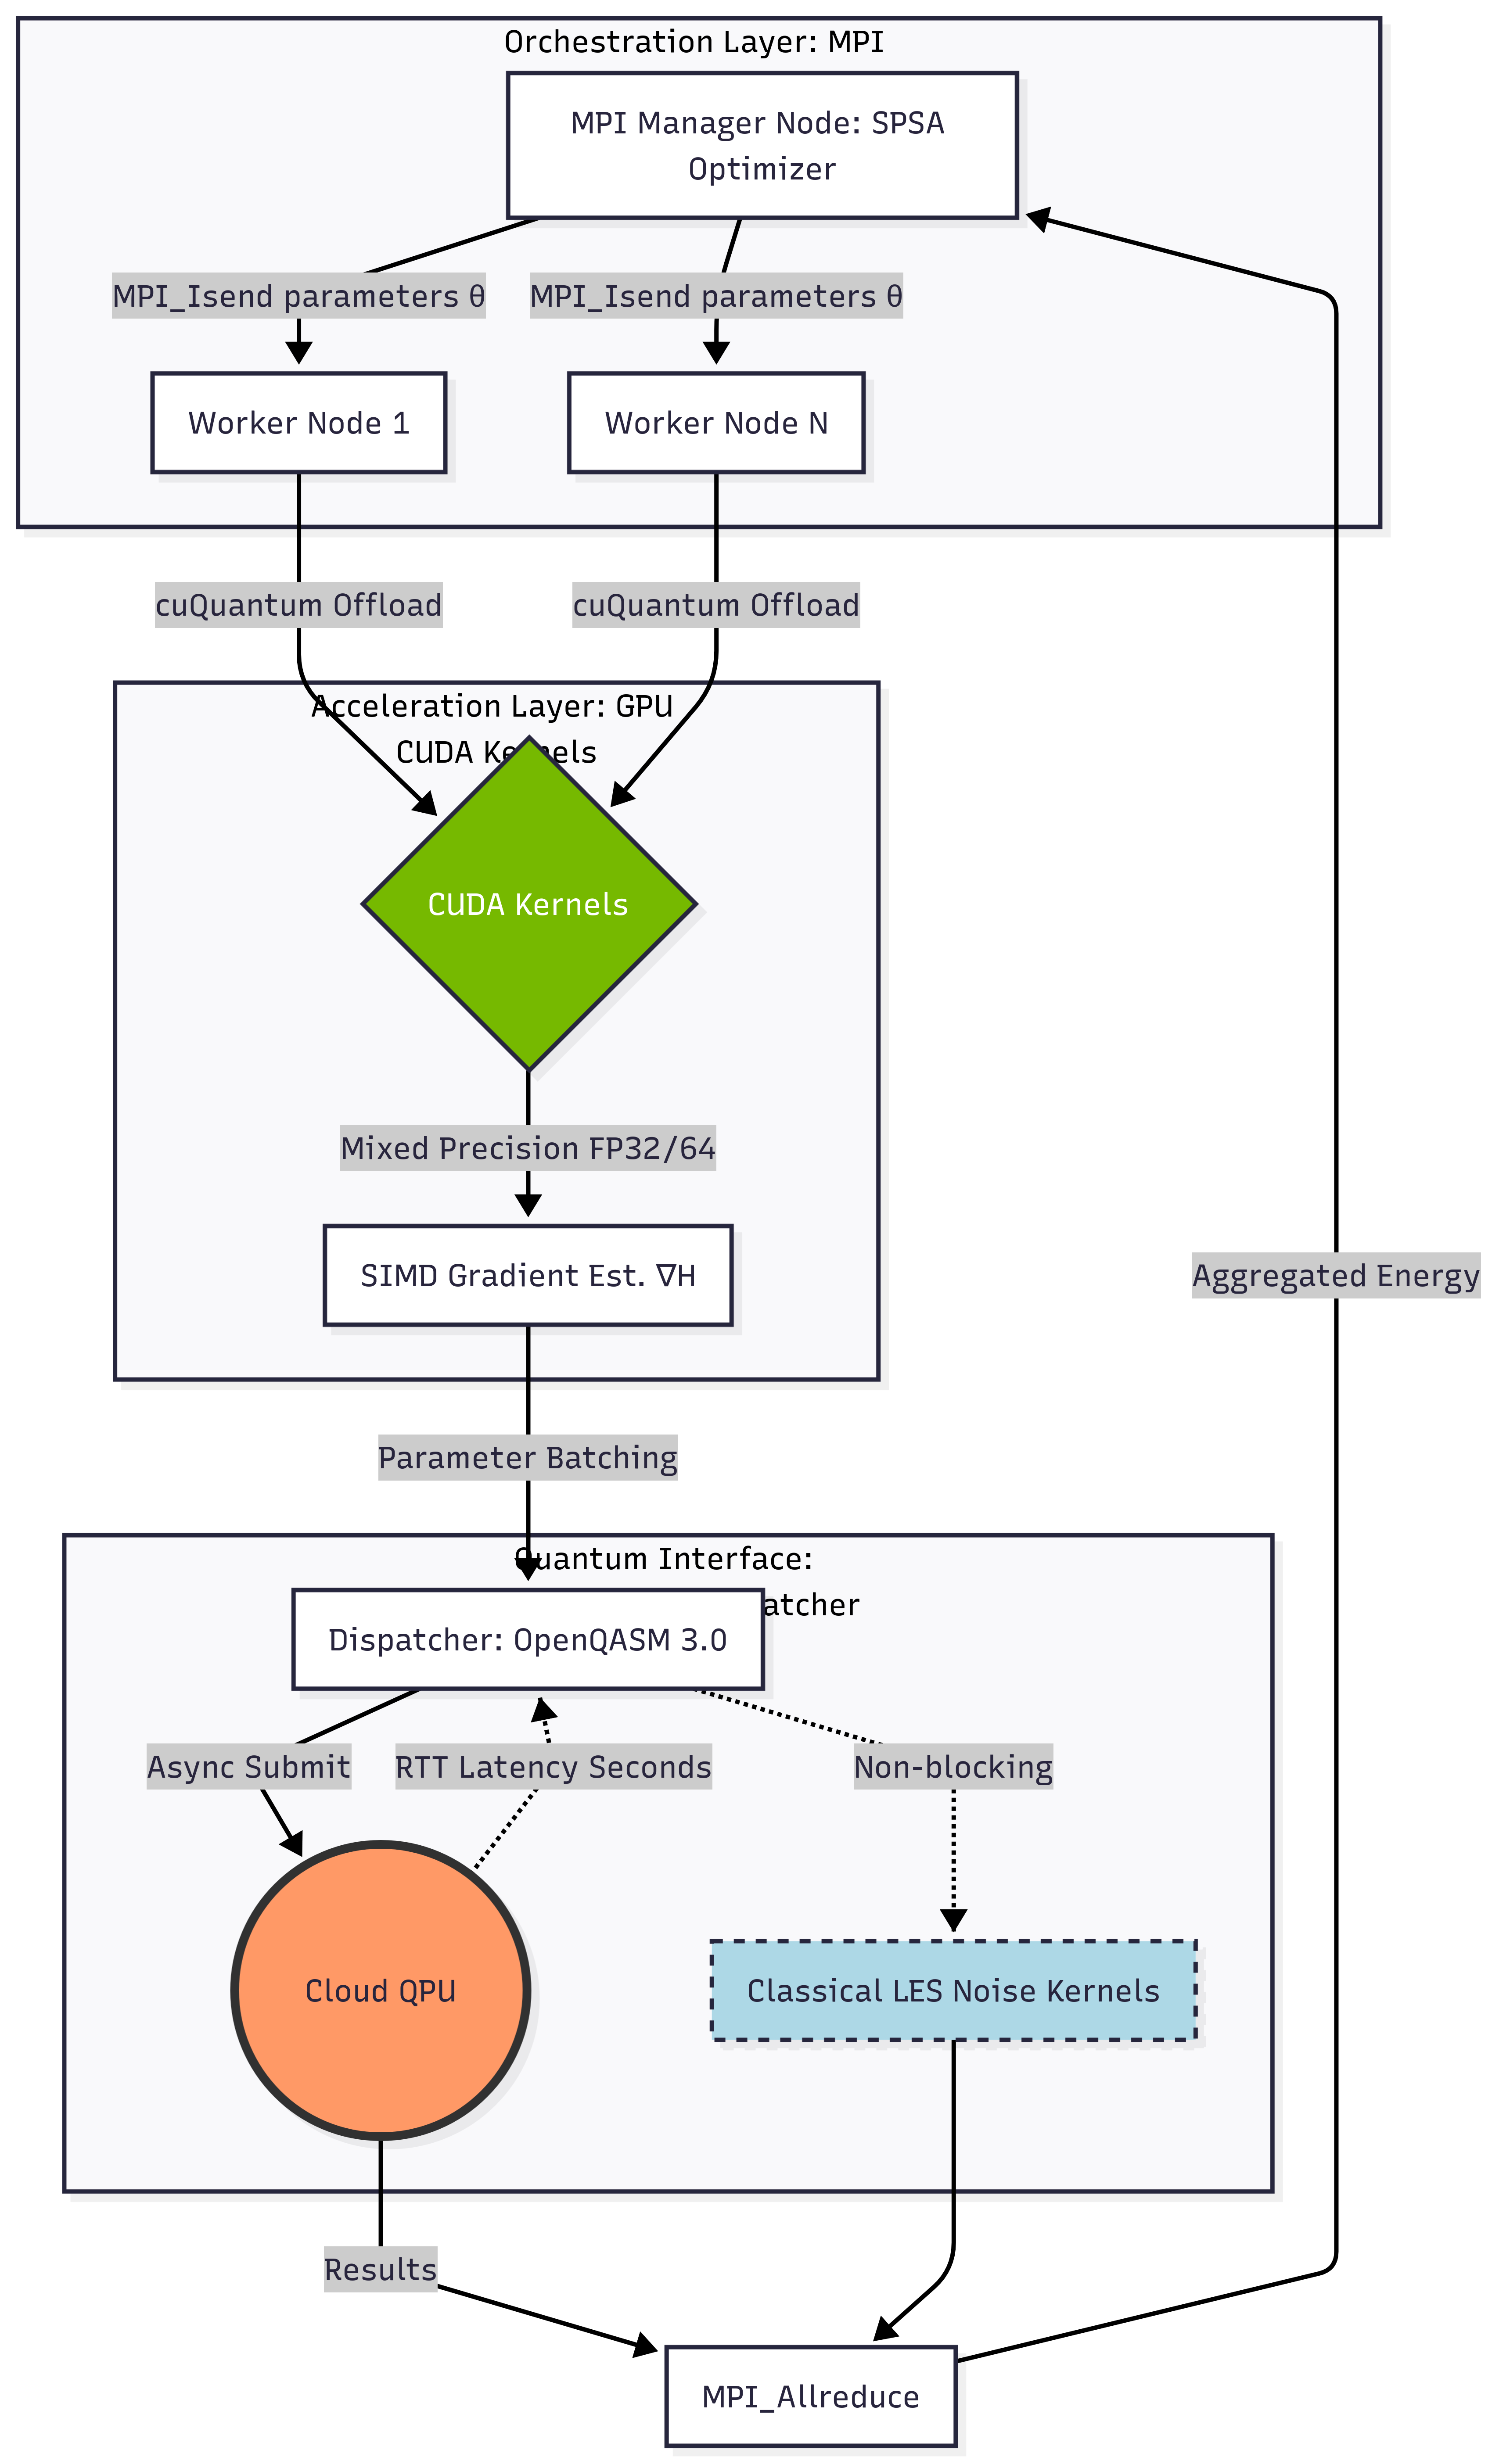
\includegraphics[width=0.8\textwidth]{graphics/system_arch_diagram.png} 
    \caption{Triple Heterogeneous System Architecture.}
    \label{fig:system_architecture}
\end{figure}


\subsubsection{Orchestration Layer: Distributed Memory and MPI Manager-Worker Topology}
This top-level layer implements a manager-worker topology that utilizes Message Passing Interface (MPI) in order to manage a cluster of compute nodes (workers). Throughout this process, the manager node handles the global state of the classical optimizer SPSA (Simultaneous Perturbation Stochastic Approximation) and distributes variational parameter sets $\theta$ across the ranks of available classical workers to enable concurrent gradient estimation. SPSA is a derivative-free optimizer, well suited to handle the quantum measurement noise found on physical qubits (unlike the gradient based methods of Adam or SGD) \cite{pellow2021classicoptimizers}. Due to this, SPSA is standard choice for VQE (and NISQ hardware) due to its ability to handle the physically noisy objective functions. 
    
By utilizing \texttt{MPI\_Isend} and \texttt{MPI\_Irecv} for non-blocking communication, the stack allows nodes to remain active and begin the local computations (such as noise modeling or basis-set transformations) while waiting for the circuit results from the cloud-based QPU. Once worker nodes receive the expectation values, they execute a \texttt{MPI\_allreduce} operation to aggregate the results and to update the global objective function. 

\begin{figure}[htbp]
    \centering
    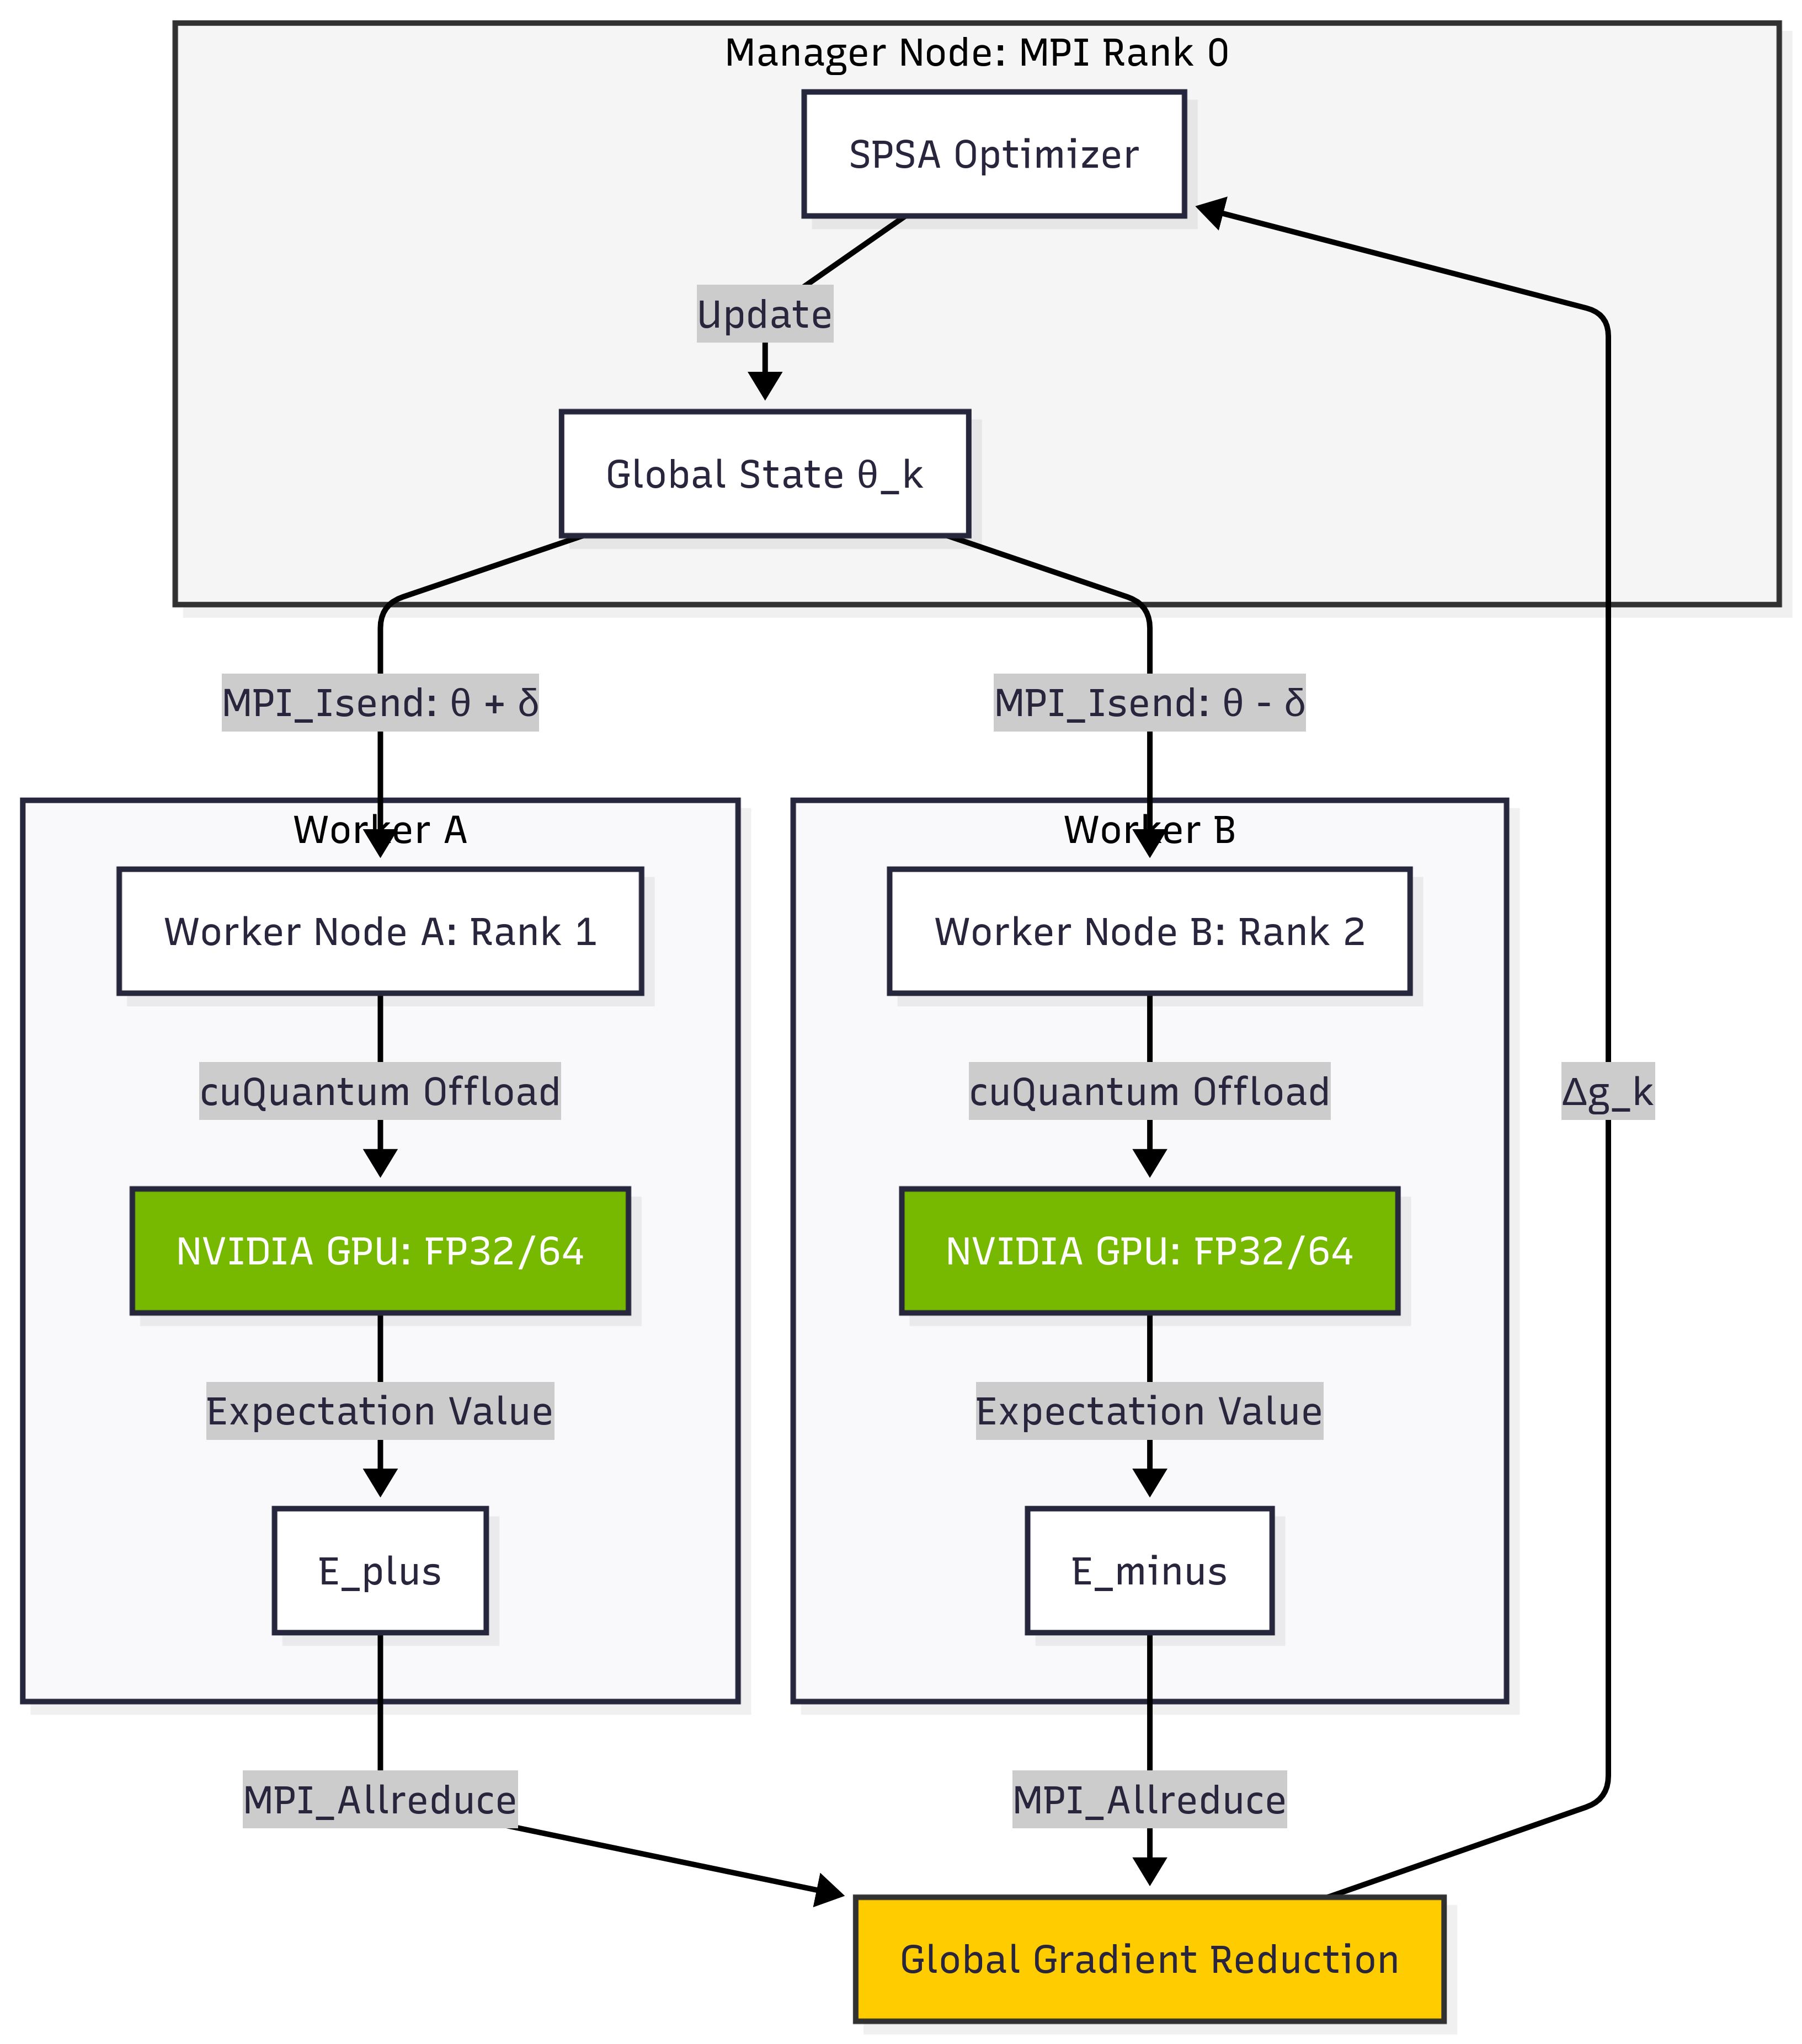
\includegraphics[width=0.8\textwidth]{graphics/spsa_topology.png} 
    \caption{Distributed SPSA Topology}
    \label{fig:spsa_topology}
\end{figure}


\subsubsection{Acceleration Layer: Intra-Node CUDA-Kernel Execution}
This layer follows the findings of Bayraktar et al. \cite{bayraktar2023cuquantum} and is designed in order to offload the computationally heavy $2^n$ state-vector math to each MPI rank's NVIDIA GPU. The stack implements a tiered acceleration strategy with an automatic fallback in place:

\begin{enumerate}
    \item \textbf{GPU statevector (cuStateVec)}: When an NVIDIA GPU is detected, the stack switches to use Qiskit Aer's GPU-accelerated statevector simulator backed by NVIDIA's cuStateVec library from the cuQuantum SDK. This accelerates the $O(2^n)$ statevector construction, which dominates per-iteration cost.
    \item \textbf{CUDA Pauli kernel}: A custom CUDA kernel computes the Pauli term expectation values using a mean-field approximation, with one GPU thread per Pauli term and tree reduction in shared memory. This kernel processes the distributed Pauli terms that are assigned to each MPI rank.
    \item \textbf{CPU fallback}: When no GPU is available, the stack falls back to Qiskit's CPU-based \texttt{Statevector} class for exact state-vector simulation. 
\end{enumerate}

The CUDA kernel adopts a Mixed Precision strategy using FP32/FP64 (32-64 bit floating-point), balancing the stacks need for high computational throughput with  numerical accuracy. FP32 (Single Precision) handles the trigonometric computations of \texttt{cosf} and \texttt{sinf} within each occuring Pauli term evaluation, which provides up to 2x faster throughput on the GPU cores. FP64 (Double Precision) is used for the implemented tree reduction and global accumulation phases in order to prevent precision loss that can occur during the summation of many small contributions. The MPI \texttt{Allreduce} aggregation also operates within FP64, ensuring that the final energy estimate maintains a full double precision accuracy across all ranks.


\subsubsection{Quantum Interface Layer - Asynchronous Dispatcher}
This layer conducts the abstraction of the hardware specific drivers and handles job submission to both local simulators and cloud based QPU backends. Two complementary dispatch paths occur:

\begin{enumerate}
    \item \textbf{C++ dispatcher} (\texttt{dispatcher.cpp}): Manages the MPI synchronization with \texttt{MPI\_Bcast} for parameter distribution and \texttt{MPI\_Allreduce} for the following energy aggregation. Routes computation to either the CUDA Pauli kernel (when GPU is available) or to the CPU mean-field fallback path. For the cloud QPU path, it uses \texttt{std::async} for non-blocking job submission via REST client (\texttt{qpu\_client.cpp}) that then handles IBM Quantum's IAM authentication, JSON payload construction, and polling with exponential backoff.

    \item \textbf{Python EstimatorV2 path} (\texttt{interface.py}): For IBM Quantum experiments, the stack uses Qiskit's EstimatorV2 primitive, which provides the stack with built-in transpilation, observable layout mapping, along with T-REx measurement error mitigation. Both the $E(\theta^+)$ and $E(\theta^-)$ gradient estimations are bundled into one job as two Primitive Unified Blocs (PUBs), therefore reducing the number of QPU round-trips by 50\%. During the QPU wait time, all MPI ranks concurrently compute exact statevector expectation values, providing both a noise-free reference estimate and useful classical work that contributes to the masking metric $M$.
\end{enumerate}

This dual path design allows the stack to determine and then utilize the most appropriate interface for each backend, chosing either the high level Python path for cloud QPU access (with its built-in error mitigation strategy), or the low level C++ dispatcher to better handle high-throughput local computation with GPU acceleration.


\subsection{Algorithmic Workflow: Parallelized VQE}
The Variational Quantum Eigensolver algorithm is reformulated in this stack in order to exploit its distributed nature, following an iterative cycle of: 

    \begin{enumerate}
        \item Global Parameter Broadcast: The optimizer rank broadcasts a vector of parameters ($\theta$) to $P$ parallel nodes.

        \item Parallel Expectation Value Estimation: Each node ($p \in P$) compute the subset of the Pauli string expectation values: $$\langle\psi(\theta)|\hat{O}_i|\psi(\theta)\rangle$$ This is the stacks primary point of parallelization in which $O_i$ terms are distributed across the HPC cluster.

        \item Asynchronous Handshake: When using the cloud QPU backend, circuits queue on the remote processor while the classical MPI ranks will concurrently compute the exact statevector expectation values locally. This overlap provides both noise-free reference estimate and classical work that masks the QPU round-trip latencies.

        \item Reduction and Updating: Expectation values get aggregated using \texttt{MPI\_Allreduce}, then the classical components compute the next $\theta$ for the following iteration.
    \end{enumerate}


\subsection{Performance Evaluation and Experimental Design}
This section describes the full evaluation of this middlware stack, validated through a Strong Scaling analysis, which measures the stack's performance when total problem size is kept fixed while the number of cores is varied \cite{cuboulderScaling}. Strong scaling measures the parallelization efficiency in a fixed environment, therefore Weak Scaling analysis is also implemented to test the middleware's communication overhead to determine if it grows sublinearly as the system scales. 


\subsubsection{Experimental Configuration}  
All simulator experiments of this stack were conducted inside of a Docker container (CUDA toolkit 12.2, Qiskit 2.1+, qiskit-ibm-runtimme 0.45.1, Python 3.11, PySCF 2.4+, OpenMPI from Ubuntu 22.04 system package) on a single host machine Intel Core i7-1065G7 (Ice Lake, with 4 physical cores and 8 logical threads) clocked at 1.30 GHz base, 3.90 GHz turbo with 32 GB RAM, running on Linux Mint. This configuration is done to ensure reproducibility across computing devices. In order to measure strong scaling under the shared memory conditions, the MPI ranks  $P \in \{1,2,4,8\}$ were evaluated on a single host and all results represent a lower bound of the speedup achievable within dedicated multi-node hardware that is connected through Infiniband. 

The SPSA optimizer of the VQE is configured with a fixed pertubation size $c = 0.1$ that can appropriately handle varational angles within $[0,2\pi]$ with a step size of $a=0.628 / \sqrt{p/8}$, which scales inversely with the square root of the number of variational parameters. $A = 0.1 \times \text{max\_iterations}$, the stability constant, delays any aggressively early updates while the decay exponents of $\alpha= 0.602$ and $\gamma = 0.101$ follow the standard schedule of SPSA. The per-iteration update rule is:
\begin{equation}
    a_k = \frac{a}{(k + A)^\alpha}, \quad c_k = \frac{c}{k^\gamma}
\end{equation}
Convergence is determined by a sliding window of 10 iterations and the optimizer terminates when $\max(E) - \min(E) < \tau$ within that window (as $\tau = 1.6$ mHa : the chemical accuracy threshold). An enforced minimum iteration count of $\max(10, \min(2p, 50))$ is applied to prevent false convergences from occuring on the small, early steps. A maximum iteration count scales alongside the number of parameters with $\max(200, 8p)$. For reproducibility, all experiments use a fixed random seed of 42. 

The ansatz configuration that is implemented within the stack is a tiered ansatz system that selects based on a correlation score metric. All four of the benchmark molecules fall within the tier of \texttt{hwe\_adaptive} tier (within correlation scores 0.34--0.50), using the EfficientSU2 circuit with full entanglement and $\min(\text{reps}+1, 3)$ number of repetition layers. The variational parameters use a uniform distribution during initialization ($\mathcal{U}(-0.1, 0.1)$), in order to keep the initial HWE state close to the Hatree-Fock reference $|0\ldots0\rangle$ under the Jordan-Wigner mapping to delay the occurance of particle number violations.  

All quantum backend experiments utilize IBM Quantum’s open access plan, which provides the 156 qubit \texttt{ibm\_marrakesh} processor. The Qiskit IBM Runtime EstimatorV2 primitive is configured with 4096 shots per circuit and with a resilience level 1 (T-REx measurement error mitigation). The GPU-accelerated experiments using NVIDIA GPUs with cuStateVec are architecturally supported within the stack's design and ADD GPU RESULTS WHEN OBTAIED.  

\subsubsection{Application Scenarios}
To demonstrate the effectiveness of this middleware when dealt a scientifically meaningful workload, this project focuses on quantum chemistry and computing the molecular electronic ground-state energies with the VQE. Chemistry was selected as the application for this middleware due three main reasons: firstly, the molecular Hamiltonian maps naturally to a qubit operator through the Jordan-Wigner transformation, which produces a clearly defined set of Pauli terms to then be distributed across MPI ranks (while still not exceeding the coherency limitations of modern day QPUs). Secondly, it was chosen due to the problem size scaling predictably with the number of electrons and basis functions to allow for controlled experiments (ranging from 4-14 qubits). Lastly, it was selected due to the prexisting Full Configuration Interaction (FCI) energies which provide verified ground-truth references for each molecule to be compared to, in order to understand the stacks accuracy. 

From the STO-3G minimal basis set, four molecules of increasing complexity were identified to be benchmark targets for this middleware. Together, these molecules progressively provide a sufficiently complex Hilbert space that can test the efficiency of the MPI/CUDA distribution while still not exceeding the coherency limitations of modern day QPUs. 

\begin{table}[htbp]
\centering
\renewcommand{\arraystretch}{1.4}
\begin{tabular}{|l|c|c|c|c|}
\hline
\textbf{Molecule} & \textbf{Electrons} & \textbf{Qubits} & \textbf{Pauli Terms} & \textbf{FCI Energy ($E_h$)} \\ \hline
H\textsubscript{2} & 2  & 4  & 15   & $-1.1373$ \\ \hline
LiH & 4  & 12 & 631  & $-7.8825$ \\ \hline
BeH\textsubscript{2}  & 6  & 14 & 666  & $-15.5951$ \\ \hline
H\textsubscript{2}O & 8  & 14 & 1086 & $-75.0124$ \\ \hline
\end{tabular}   
\caption{Benchmark molecules with STO-3G basis.  FCI energies computed with the PySCF Full Configuration Interaction solver.}
\label{table:molecules}
\end{table}   

The progression that occurs from the molecule $H_2$ (4 qubits, 15 Pauli terms - fits within the memory of a single MPI rank) to $H_{2}O$ (14 qubits, 1086 Pauli terms) stresses each layer of the middleware. This includes parameter broadcasting, Pauli term partitioning, statevector construction, and MPI reduction. 

   


\subsubsection{Scaling Strategy}
The objective of Strong Scaling is to reduce the execution time within a fixed total problem size by increasing the number of processors, while considering the ideal time spent on $N$ cores and efficiency. The formula for Ideal Time on N number of cores is \cite{cuboulderScaling}: 
\begin{equation}
    \text {Ideal Time } = \frac{(\text{Measured Time at Lowest Core Count})\text{(Lowest Core Count)}}{N}
\end{equation}

Efficiency provides the metric for the appropriate number of cores for a particular calculation size. Achieving  100\% is often not possible within practice, so a there is a tradeoff point established between the efficiency of the usage of computational resources and of the time spent waiting on the calculations to completed must be determined. The formula for Efficiency is \cite{cuboulderScaling}: 
\begin{equation}
    \text {Efficiency } = \frac{\text{Ideal Time}}{\text{Measured Time}}
\end{equation}

In addition to Strong Scaling, Weak Scaling is evaluated, where the molecule (and Hamiltonian's Pauli term count) is increased proportionally alongside the number of MPI nodes ($P$). At each rank count, a molecule is selected that ensure the per-rank workload (terms/rank) remains approximately constant: $H_{2}$ at $P=1$ (15 terms/rank), $LiH$ at $P=2$ (316 terms/rank), $BeH_{2}$ at $P=4$ (167 terms/rank), and $H_{2}O$ at $P=8$ (136 terms/rank). This will test whether the middleware maintains a stable compute-to-communication ratio while the inputted problems scales up towards the `Communication Wall.'


\subsubsection{Stress Test Design}
To ensure a robust asynchronous dispatcher and manager-worker topology, the system will undergo three evaluations using simulations for "Failure Mode": 
\begin{enumerate}
    \item QPU Latency Spiking: A variable delay will be inserted (between 5-30s) into a subset of the worker-rank network calls, done to simulate increased cloud backend latency. This will test the manager ranks ability to rebalance workloads or to be able to maintain a global synchronizations without rank timeouts. 
    \item Mixed Precision Stability: The VQE iterations will raise the number of qubits (approaching 30 qubits) within the simulation in order to monitor the vanishing gradient often caused by FP32 rounding errors. This will determine the threshold at which the system must transition itself to FP64. 
    \item Network Drop-Out Recovery: An intentional SIGKILL will be sent to a worker rank during active job submission to test if the Orchestration Layer can perform a "checkpoint restart", in where the last know global $\theta$ state that is stored in the manager rank is used to resume optimization without a full system crash. Each 5 iterations a checkpoint is saved within checkpoints/ to provide the restart points. 
\end{enumerate}


\subsection{Benchmarking and Measurement Plan}
\subsubsection{Baseline Implementations}
In order to verify the optimized performance of the triple heterogeneous stack, the system is measured against two distinct baselines: 
     \begin{itemize}
         \item Standard Serial Baseline: Execution using Qiskit Statevector VQE on a single core CPU, using identical SPSA hyperparameters, the HWE-adaptive ansatz, and the same convergence criteria as the distributed MPI/GPU stack. This identifies the outcome of the MPI distribution from any algorithmic differences, providing a fair wall-clock comparison that represents the nonoptimized and industry standard starting point.
     \end{itemize}
     \begin{itemize}
         \item Single Node GPU Baseline: Execution using cuStateVec on a single NVIDIA GPU without the MPI distribution, with this baseline done to isolate the speedup contribution from GPU acceleration vs. the multi-node MPI orchestration. ADD HERE ONCE GPU ACCESS IS OBTAINED
     \end{itemize}
 

\subsubsection{Quantitative Metrics}
The primary metric for determining the success of this stack is the observed End-to-End Wall-Clock Time ($T_{total}$). 
   \begin{equation}
    T_{\text{total}} = T_{\text{accel}} + T_{\text{comm}} + T_{\text{quant}}
\end{equation}
Where: 
\begin{itemize}
    \item $T_{accel}$ = time spent on GPU accelerated optimization (classical acceleration).
    \item $T_{comm}$ = overhead from network RTT and MPI synchronization (communication latency).
    \item $T_{quant}$ = QPU execution time (sampling and measurement).
\end{itemize}

\noindent If the quantity of metric $T_{comm}$ is successfully "masked" by the value of the asynchronous $T_{accel}$ execution time, there will be evidence of this stack's progress towards the "quantum advantage" and achievement of the targeted 1.5-3x speedup over standard single node Qiskit workflows.   

\noindent Masking Efficiency ($M$) will be used as a metric for how well the RTT is hidden (masked). 
\begin{equation}
    M= \frac{T_{\text{accel}}}{T_{\text{comm}}}
\end{equation}
If $M \ge 1$, then the classical components completely cover (mask) the communication wait time. 

\noindent To measure the system's ability to handle high volume iterative workloads, Throughput (Circuits per Second) is established as:
\begin{equation}
        \text{Throughput} = \frac{N_{\text{circuits}}}{T_{\text{total}}}
\end{equation}

\begin{table}[htbp]
\centering
\renewcommand{\arraystretch}{1.5} 
\begin{tabular}{|>{\raggedright\arraybackslash}p{3.5cm}|>{\raggedright\arraybackslash}p{1.5cm}|>{\raggedright\arraybackslash}p{4.5cm}|>{\raggedright\arraybackslash}p{3.5cm}|}
\hline
\textbf{Category} & \textbf{Metric} & \textbf{Definition} & \textbf{Success Threshold} \\ \hline
\textbf{System Performance} & $T_{total}$ & End-to-End Wall-Clock Time  & 2--3x speedup vs. Serial Baseline \\ \hline
\textbf{Latency Masking} &   $M$ & Ratio of $T_{accel} / T_{comm}$ & $M \geq 1$ (Full overlap) \\ \hline
\textbf{Throughput} & CLOPS & Circuit Layer Operations Per Second &  $>$ Qiskit serial baseline \\ \hline
\textbf{Hardware Efficiency} & $E$ & Parallel Efficiency ($S/P$) & $\geq 70\%$ at $P=2$ \\ \hline
\textbf{Resource Utilization} & $U_{gpu}$ & Average GPU Occupancy & $\geq 80\%$ during $T_{accel}$ \\ \hline
\textbf{Scientific Fidelity} & $\Delta E$  & Absolute Energy Error (Chemistry) & $\leq 1.6$ mHa (Chemical Accuracy) \\ \hline
\textbf{Resilience} & $R_{time}$ & Recovery Time after Node Failure & $<$ 60 s (Auto checkpoint) \\ \hline
\end{tabular}
\caption{Quantitative Success Metrics for Middleware Evaluation.}
\label{table:success_metrics}
\end{table}


\subsubsection{Parallel Efficiency and Scalability}
This project measures Parallel Efficiency ($E$), calculated as:
\begin{equation}
    E = \frac{S}{P} = \frac{T_{s}}{P \times T_{p}}
\end{equation}
where $P$ represents the number of active MPI nodes, $T_{s}$ is the serial (single core) wall-clock time, $T_{p}$ is the measured parallel wall-clock time, and $S = T_{s}/T_{p}$ is the measured speedup. This metric is used to demonstrate if the "Communication Wall" is being successfully handled as the cluster scales.  

\subsubsection{Correctness and Convergence}
For the purpose of ensuring the optimizations (such as Mixed Precision (FP32/FP64) and SPSA) do not compromise the science of this stack, the tested molecules ground state energy results will be compared against the preestablished Full Configuration Interaction (FCI) results for ground state energies. This software stack is considered successful within the application of quantum chemistry if it maintains Chemical Accuracy ($\approx 1.6$ mHa) throughout the parallelized iterations. 

For broader applications of this software's accuracy, Relative Error  ($\epsilon$) is used: 
\begin{equation}
    \epsilon = \frac{|E_{exact} - E_{stack}|}{|E_{exact}|} 
\end{equation}
This provides an application agnostic accuracy measure that will extends beyond quantum chemistry to any domain (future applications can include Optimization Problems, Fianancial Portfolios, etc.) where the stack can compute variational ground state energies. 





\section{Experiments}
This section provides the experimental procedures used in the evaluation of each layer of the hybrid software stack. All experiments used a fixed random seed ($\texttt{seed}=42$) in the SPSA optimizer in order to ensure reproducibility. Results are reported as the \emph{best physical energy}, which is the lowest energy observed during the optimization, remaining at or above the FCI ground truth. This addresses the HWE ansatz's tendency of exploring unphysical Hilbert space sectors (discussed in Section~\ref{sec:hwe_limitation}).

\subsection{Experiment 1: Distributed Statevector VQE (Simulator)}
The objective of this experiment is to validate the distributed statevector evaluation path to produce physically correct ground-state energy estimates, then to compare the accuracy against the serial baseline's.

\subsubsection{Procedure}
In this experiment, each presented molecule from Table \ref{table:molecules} was optimized using the following identical configuration:

\begin{itemize}
    \item \textbf{Backend}: Statevector simulator (exact, noiseless)       
    \item \textbf{MPI ranks}: $P = 2$                     
    \item \textbf{Ansatz}: HWE-adaptive (EfficientSU2, full entanglement, auto selected reps)
    \item \textbf{Optimizer}: SPSA with dimension scaled step size ($a = 0.628 / \sqrt{n_{\text{params}} / 8}$)
    \item \textbf{Max iterations}: $\max(200,\; n_{\text{params}} \times 8)$, scaling with problem dimension
    \item \textbf{Convergence}: Energy spread over the last 10 iterations $< 1.6 \times 10^{-3}$ Ha        
    \item \textbf{Initialization}: Parameters drawn from $\mathcal{U}(-0.1, 0.1)$, keeping the initial state near the Hartree-Fock reference $|0\ldots0\rangle$
\end{itemize}   

Pauli terms of the molecular Hamiltonian were partitioned evenly across MPI ranks, where each rank independently established $2^n$-dimensional statevector and then evaluated its local subset of $\langle\psi(\theta)|O_i|\psi(\theta)\rangle$ terms. A global \texttt{MPI\_Allreduce(SUM)} aggregated the partial energies and the masking metric $M = T_{\text{accel}} / T_{\text{comm}}$ was recorded one time per iteration.

\subsubsection{Serial Baseline}
An identical VQE was executed within a single Python process without using MPI, however maintaining the same ansatz, SPSA parameters, seed, and convergence criteria. This then provides the $T_{\text{serial}}$ value for speedup calculations. Note that the serial baseline may converge at a different iteration count than the distributed stack (e.g., $LiH$ serial converged in 576 iterations vs. 768 for the distributed path), as the convergence criterion can trigger earlier or later depending on the stochastic SPSA trajectory in each execution path.


\subsection{Experiment 2: Strong Scaling Analysis}
The objective of this experiment is to measure how the wall clock time decreases while the number of MPI ranks increases in a fixed problem size, and determines the communication-to- computation ratio.     

\subsubsection{Procedure}
All four benchmark molecules (Table~\ref{table:molecules}) were run at full iteration counts for each rank count $P \in \{1,2,4,8\}$, all within one Docker container on a single host. $H_{2}O$ (14 qubits, 1086 Pauli terms, 896 iterations) was selected as the primary efficiency benchmark due to having the largest number of distributable Pauli terms. Parallel efficiency was then computed as:
\begin{equation}
    E(P) = \frac{T_1}{P \times T_P}
\end{equation}         
where $T_1$ is the determined wall clock time at $P=1$.     


\subsection{Experiment 3: IBM Quantum QPU Validation}   
This exeriment is done to demonstrate the end-to-end middleware functionality when using a real quantum processor (QPU). This experiment validates the Python EstimatorV2 integration, transpilation pipeline, and the MPI coordination with cloud-based QPU results.

\subsubsection{Procedure}   
The molecule $H_{2}$ was selected to be inputted in the IBM QPU experiment due to it requiring the least amount of qubits (4 qubits) out of the 4 molecules tested. This VQE was configured with:  

\begin{itemize}
    \item \textbf{Backend}: IBM \texttt{ibm\_marrakesh} (156 physical qubits)
    \item \textbf{MPI ranks}: $P = 2$ (rank 0 manages QPU submission)
    \item \textbf{Shots}: 4096 per circuit   
    \item \textbf{Error mitigation}: T-REx (resilience level 1)
    \item \textbf{Max iterations}: 10
    \item \textbf{Job batching}: Both $E(\theta^+)$ and $E(\theta^-)$ were submitted as 2 Primitive Unified Blocs (PUBs) within a single EstimatorV2 job, reducing the queue wait by 50\%
\end{itemize}

Here, the ansatz was transpiled once against the backend's coupling map by using Qiskit's preset pass manager (optimization level 1). The observable was then remapped to the physical qubit layout. On IBM's open access plan, Sessions are not supported, so each iteration submits an independent job via the sessionless EstimatorV2 mode. The transpiled circuit and observable layout are cached locally and reused across iterations to avoid redundant compilation.    

Results for this are presented in Tables~\ref{table:ibm_results} and~\ref{table:ibm_iterations}.

\subsection{Experiment 4: GPU-Accelerated Statevector}

% TODO-GPU: Add experimental procedure for cuQuantum integration benchmarks.
% Procedure: Run make run NP=2 with USE_GPU=yes on a node with NVIDIA A100/V100.
% Compare: GPU statevector build time vs CPU, per-iteration wall time, scaling at P=1,2,4,8.
% Record: GPU occupancy via nvprof/nsight, memory bandwidth utilization.


\subsection{Experiment 5: Checkpoint Resilience}
This exerpiment is conducted to validate the checkpoint restart mechanism, which verifes optimization can resume from the saved $\theta$ state without a loss of convergence progress.

\subsubsection{Procedure}
A 6 layer diagnostic test (\texttt{test\_layers\_run.py}) within the stack executes this automatically: 

\begin{enumerate}
    \item Run $H_{2}$ VQE for 5 iterations, then save checkpoint.
    \item Verify the checkpoint file exists and contains the correct parameter vector shape.
    \item Restart VQE from the checkpoint, running 5 additional iterations (6-10). 
    \item Verify the optimizer resumes from correct SPSA schedule position ($k=6$) and that the restarted energy continues on from the checkpointed trajectory.
\end{enumerate}  


\pagestyle{fancy} 
\section{Results}

This is your results section text


\pagestyle{fancy} 
\section{Discussion}

This is your discussion text




\section{Future Work}
\label{sec:future}

There are several extensions taht would strengthen the current implementations of this middleware stack in the hopes of broadening its applicability, speed, and accuracy:

\subsection{Particle-Number-Conserving Ansatzes}
The HWE ansatz used in this work does not conserve particle number in the way a UCC ansatz would, which in our results led to unphysical energy estimates dropping below FCI, even after sufficient SPSA iterations. Therefore, in the ongoing development of this stack, we have begun the integration of the Unitary Coupled Cluster Singles and Doubles (UCCSD) ansatz, which will preserves particle number. UCCSD is already architecturally supported in an ansatz tier system, with integration ongoing due to the stack encountering compatibility challenges, specifically Qiskit Nature's gate decomposition pipeline. Resolving this issue would eliminate the need for the current approach of the stack of tracking best-physical-energy and could produce physically correct results that satisfy the variational principle throughout optimization.

\subsection{Advanced Quantum Error Mitigation}
The IBM QPU experiments used only T-REx (resilience level 1), which only handles measurement readout errors but not the potential quantum gate errors or expected qubit decoherence. Here, integration with Zero Noise Extrapolation (ZNE) or Probabilistic Error Cancellation (PEC) with Qiskit's provided option of resilience level 2+ is predicted to significantly improve the QPU accuracy without hardware changes. Currently, the stack's EstimatorV2 integration supports these with \texttt{options.resilience\_level} parameter.

\subsection{Multi Node Scaling with InfiniBand}
All current scaling experiments for this stack were conducted on a single Docker host with MPI ranks sharing the CPU cores and memory bandwidth. Deploying on a multi-node cluster with efficient InfiniBand interconnect would eliminate shared memory contention that was observed at $P \geq 4$ and will provide a improved measurement of the stack's scaling abilities.

\subsection{Application Extensibility}
The stack currently includes a \texttt{FinanceProblem} class which maps portfolio optimization to a QUBO/Ising Hamiltonian, demonstrating that in the future this middleware will notbe limited solely to quantum chemistry. Future work will extending the current stack appplications to include combinatorial optimization (MaxCut, TSP) and materials science (periodic Hamiltonians), done through leveraging the same MPI distribution/QPU dispatch infrastructure. This application agnosticism will further set apart this stack from others such as XACC, which focuses solely on the mapping of quantum chemistry.

\subsection{Hardware Portability}
Following the previous XACC approach of ensuring hardware agnostic QPU access (allowing a hardware plug-in option for several QPUs of different companies), this stack will be extended in the future to support additional quantum backends (such as Amazon Braket, Azure Quantum, IonQ) by additional dispatcher plugins. The current dual path architecture (the C++ dispatcher for stack MPI coordination, Python primitives for QPU access) already provides a natural extension point for this task.


\pagestyle{fancy} 
\section{Conclusion}

This is your conclusions

\begin{appendices}

Your supplementary materials are placed here.

\end{appendices}

\printbibliography

\end{document}
